\chapter{Realizability}
\label{chap:realizability}

\section{The basic idea and definition}
\label{sec:realizability-basic-idea}

Given a mathematical structure (constants, functions, relations, and
axioms), what should a computer implementation look like? For simple
cases, the answer is obvious. A group would have a type whose values
represent group elements, a value representing the neutral element,
and functions which compute the group operation and inverses. But for
more interesting structures, especially those arising in mathematical
analysis, the answer is less clear. How do we implement the real
numbers (and we do not mean floating-point arithmetic, we mean the
\emph{real} real numbers)? Which operations on a compact metric space
can be implemented? How do we implement a space of smooth functions?
Significant research goes into finding satisfactory answers to such
questions~\cite{Wei00,TZ98,Bla97}.

To explain the basic idea behind realizability we consider a small
real-world programming example. Suppose we are asked to design a data
structure for the set $\mathsf{Graphs}$ of all finite
simple\footnote{Simple means at most one arrow between any two
  vertices.} directed graphs with vertices labeled by distinct
integers. An typical such graph~$G$ is shown in
Figure~\ref{fig:digraph}.
%
\begin{figure}[htp]
  \centering
  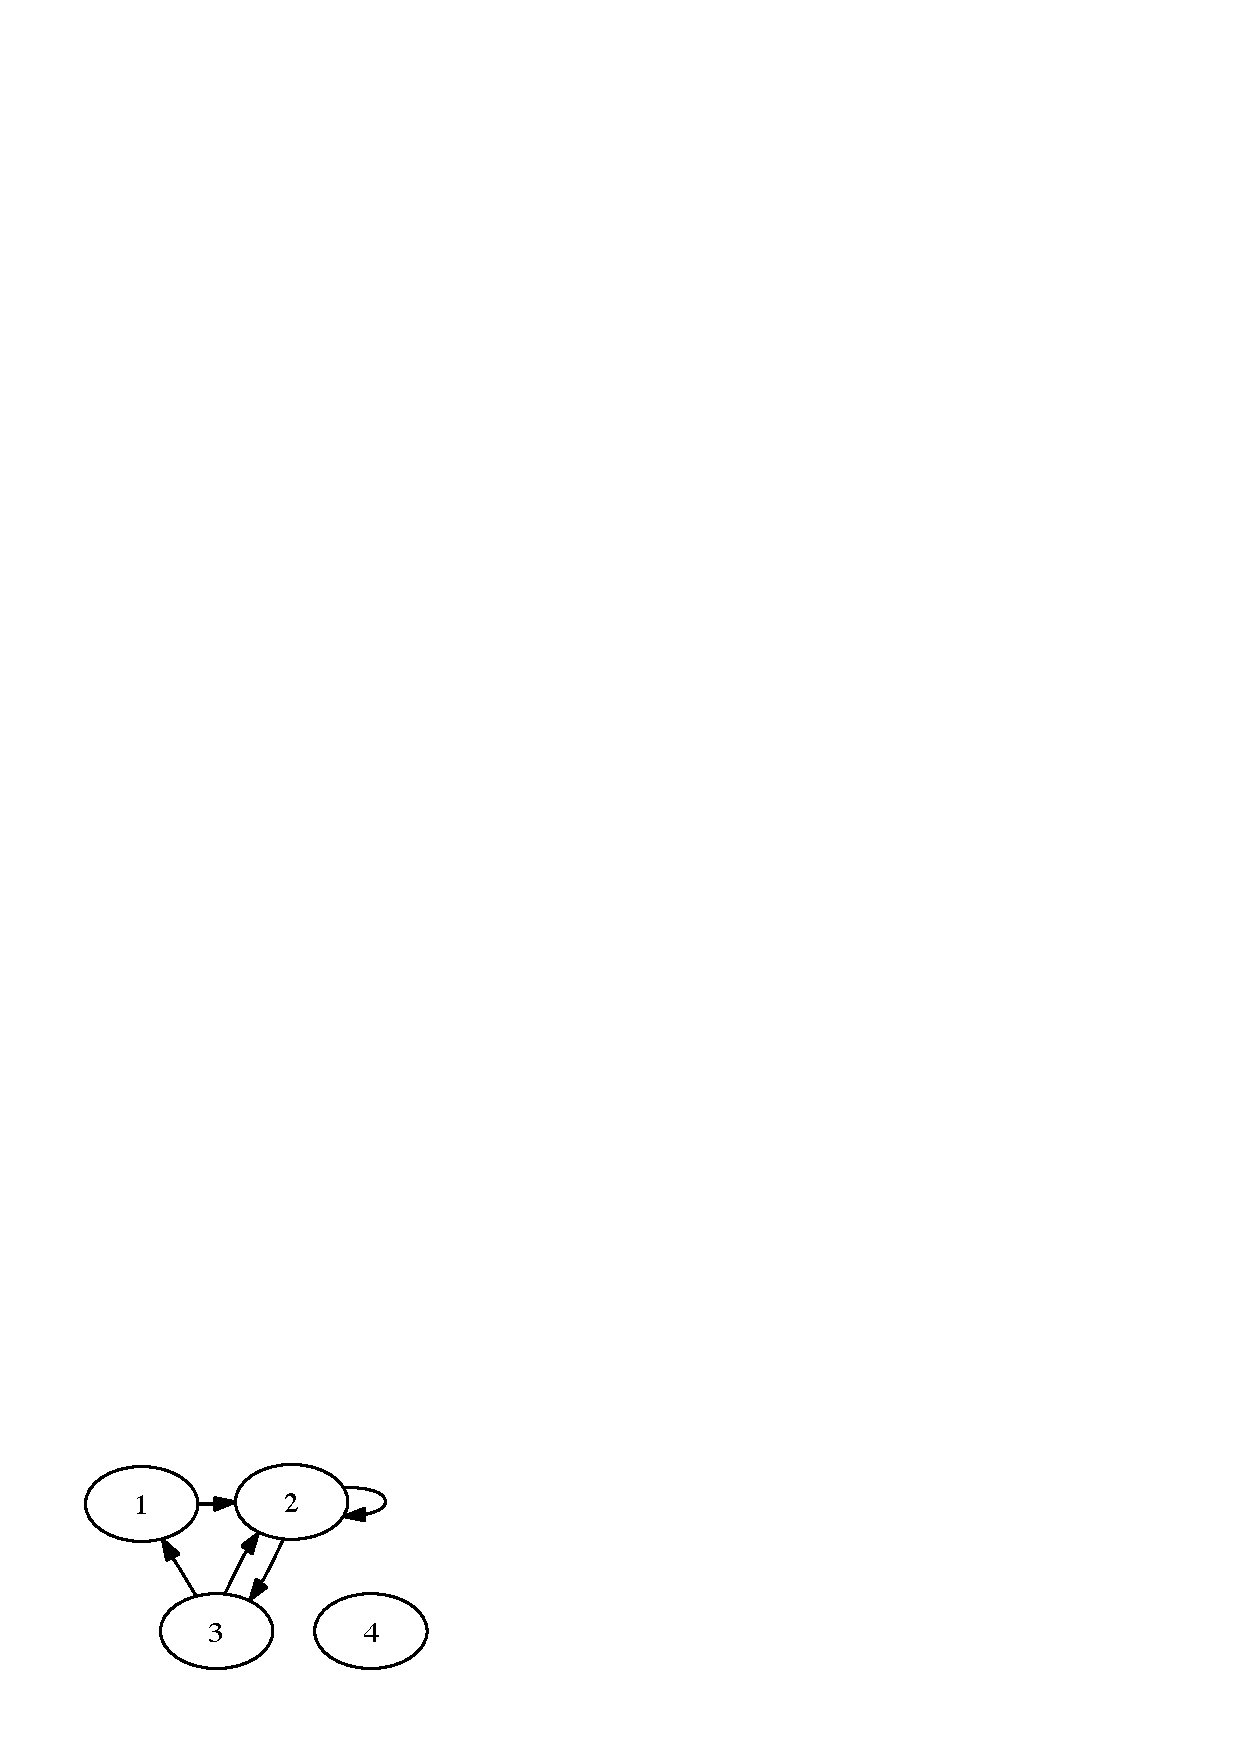
\includegraphics[width=0.3\textwidth]{digraph}
  \caption{A finite directed graph $G$}
  \label{fig:digraph}
\end{figure}
%
One common representation of such graphs uses a pair of lists
$(\ell_V, \ell_A)$, where $\ell_V$ is the list of vertex labels and
$\ell_A$ is the \emph{adjacency list} representing the arrows by
pairing the labels of each source and target. For the above graph $G$,
$\ell_V = [1, 2, 3, 4]$ and $\ell_A = [(1,2), (2,2), (2,3), (3,2),
(3,1)]$.
%
Thus we define the datatype of graphs as\footnote{We use Haskell
  notation in which $[t]$ is the type of lists of elements of
  type~$t$, and $(t_1, t_2)$ is the cartesian product of types~$t_1$
  and~$t_2$.}
%
\begin{lstlisting}[language=Haskell]
type Graph = ([Int], [(Int, Int)])
\end{lstlisting}
%
However, this is not a complete description of the intended
representation, as there are representation invariants and conditions
not expressed by the type, e.g.,
%
\begin{enumerate}
\item The order in which vertices and arrows are listed is not
  important%
; for example, $[1,2,3,4]$ and $[4,1,2,3]$ represent the same vertices.
\item Each vertex and arrow must be listed exactly once.
\item The source and target of each arrow must appear in the list of vertices.
\end{enumerate}
%
Thus, to implement the mathematical set~$\mathsf{Graphs}$, we must not
only decide on the underlying datatype $\mathtt{graph}$, but also
determine what values of that type represent which elements
of~$\mathsf{Graphs}$. All this can be expressed with a \emph{realizability
  relation}
%
\begin{equation*}
  r \rz x
\end{equation*}
%
which is read as ``$r$ realizes $x$''. In the above example we would
write
%
\begin{equation*}
([1, 2, 3, 4], [(1,2), (2,2), (2,3), (3,2), (3,1)]) \rz G.
\end{equation*}
%
We now give a precise definition.


\begin{definition}[Assemblies]
  Let $A$ be a TPCA and $\comp{A}$ a sub-TPCA. An \emph{assembly}
  over~$(A, \comp{A})$ is a triple $(S, |S|, {\rz_S})$ where $S$ is a
  set, $|S|$ is a type, and $\rz_S$ is a relation between $A_{|S|}$
  and~$S$ satisfying: for every $x \in S$ there is $r \in A_{|S|}$
  such that $r \rz_S x$.

  A \emph{realized map} $f : S \to T$ between assemblies $(S, |S|,
  {\rz_S})$ and $(T, |T|, {\rz_T})$ is a map for which there exists $p
  \in \comp{A}_{|S| \to |T|}$ satisfying: if $r \rz_S x$ then $\defined{p
    \cdot r}$ and $p \cdot r \rz_T f(x)$.

  Assemblies and realized maps form the \emph{category
    $\Asm{A,\comp{A}}$ of assemblies over $(A, \comp{A})$}.
\end{definition}

\noindent
There are many versions of realizability. Ours is known as \emph{typed
  relative realizability}. It is typed because we used typed PCAs
rather than the ordinary ones. It is relative because we used one
TPCA~$A$ for assemblies, and another for the realized maps. By this we
are capturing the idea that computable functions may operate on
potentially non-computable data, as was the case for type~2 machines
and the graph model, cf.\ Sections~\ref{sec:type-2}
and~\ref{sec:graph-model}. In the typical case the larger TPCA~$A$
allows representation of arbitrary data, but the sub-TPCA $\comp{A}$
consists only of the computable part of~$A$ which forces the realizers
for maps to be computable. Thus it makes sense to say in the general
case that the maps are realized \emph{relative} to the choice of a
sub-TPCA~$\comp{A}$.

When $A$ is not typed the definition of an assembly simplifies a bit
because we need not keep mentioning the (trivial) types: an assembly
over a PCA~$A$ is a pair $(S, {\rz_S})$ where $S$ is a set and $\rz_S$
is a relation between~$A$ and~$S$, such that for every $x \in S$ there
is $r \in A$ and $r \rz_S x$.

Another special case occurs when $\comp{A} = A$. In this case we write
$\Asm{A}$ instead of $\Asm{A,A}$.

Normally the TPCA $A$ will actually be an NR-TPCA, and $\comp{A}$ a
sub-NR-TPCA of~$A$.

Particular choices of a TPCA with sub-TPCA yield well known ``schools
of computable mathematics'':
%
\begin{enumerate}
\item When $A = \comp{A} = \NN$ is the first Kleene algebra we get the
  Russian school of \emph{recursive
    mathematics}~\cite{recursive-math}, also known as \emph{type I
    computability} because the underlying computational model is that
  of type~1 machines.
\item When $A = \Baire$ is the second Kleene algebra we get Kleene's
  \emph{function realizability}~\cite{KleeneSC:fouim}, also known by
  its newer name \emph{type two effectivity (TTE)}~\cite{tte}. There
  are actually three variants:
  %
  \begin{enumerate}
  \item $A = \comp{A} = \Baire$ is \emph{continuous} function
    realizability because maps are realized by arbitrary continuous
    realizers,
  \item $A = \Baire$ and $\comp{A} = \comp{\Baire}$, where
    $\comp{\Baire}$ is the set of computable sequences, is the
    \emph{relative} type 2 realizability,
  \item $A = \comp{A} = \comp{\Baire}$ is the \emph{computable}
    function realizability.
  \end{enumerate}
  %
  We will mostly study the continuous and the relative function
  realizaiblity.
\item When $A = \Scott$ is the graph model we get a version of
  realizability that is closely related to equilogical
  spaces~\cite{BauerA:equs}. Here two there are three variants:
  %
  \begin{enumerate}
  \item $A = \comp{A} = \Scott$ is the continuous model,
  \item $A = \Scott$ and $A = \comp{\Scott}$ is the family of
    c.e.~sets is the relative model,
  \item $A = \Scott = \comp{\Scott}$ is the computable model.
  \end{enumerate}
\item Closely related to the previous case is $A = U$ where~$U$ is a
  universal Scott domain~\cite{GunterScott}. This again gives as three
  variants of \emph{domain representations}~\cite{Bla97,Bla97a}.
\item The case $A = \PCFinf$ and $\comp{A} = \PCF$, cf.
  Section~\ref{sec:pcf} is interesting because we may actually test
  the performance of PCF realizers by running them as Haskell
  programs.
\end{enumerate}
%
In Section~\ref{variants} we shall study some of these in greater
detail.




\section{Equivalent formulations}
\label{sec:representations-formulations}

\subsection{Assemblies and modest sets}
\label{sec:assemblies}

\subsection{Partial equivalence relations}
\label{sec:pers}

\subsection{Representations}
\label{sec:representations}


\section{Type 1 representations}
\label{sec:type-1-representations}

\section{Type 2 representations}
\label{sec:tte-representations}

Admissibility.

\section{Equilogical spaces and domain representations}
\label{sec:equilogical-spaces}

\section{A convenient category of spaces}
\label{sec:qcb-spaces}



%%% Local Variables: 
%%% mode: latex
%%% TeX-master: "notes"
%%% End: 
